% \begin{theo}[Rotationele grootheden]{Rotationele grootheden}
%     \begin{minipage}{.56\textwidth}
%         \begin{itemize}
%             \item \textbf{Hoekverplaatsing:} $ \Delta \theta = \theta_2 - \theta_1 $
%             \item \textbf{Hoek:} $ \theta = \dfrac{\ell}{R}$  
%             \item \textbf{Hoeksnelheid:} $ (= \dfrac{\text{rad}}{s})$
%             \begin{itemize}
%                 \item \textbf{Gemiddelde:} $ \omega_{gem} = \dfrac{\Delta\theta}{\Delta t}$
%                 \item \textbf{Ogenblikkelijke:} $ \omega = \lim_{\Delta t \to 0} \dfrac{\Delta\theta}{\Delta t} = \dfrac{d\theta}{dt} $ 
%             \end{itemize}
%             \item \textbf{Hoekversnelling:} $ (= \dfrac{\text{rad}}{s^2}) $
%             \begin{itemize}
%                 \item \textbf{Gemiddelde:} $ \alpha_{gem} = \dfrac{\Delta\omega}{\Delta t}$
%                 \item \textbf{Ogenblikkelijke:} $ \alpha = \lim_{\Delta t \to 0} \dfrac{\Delta\omega}{\Delta t} = \dfrac{d\omega}{dt} $ 
%             \end{itemize}
%         \end{itemize}
%     \end{minipage} 
%     \begin{minipage}{.40\textwidth}
%         \centering
%         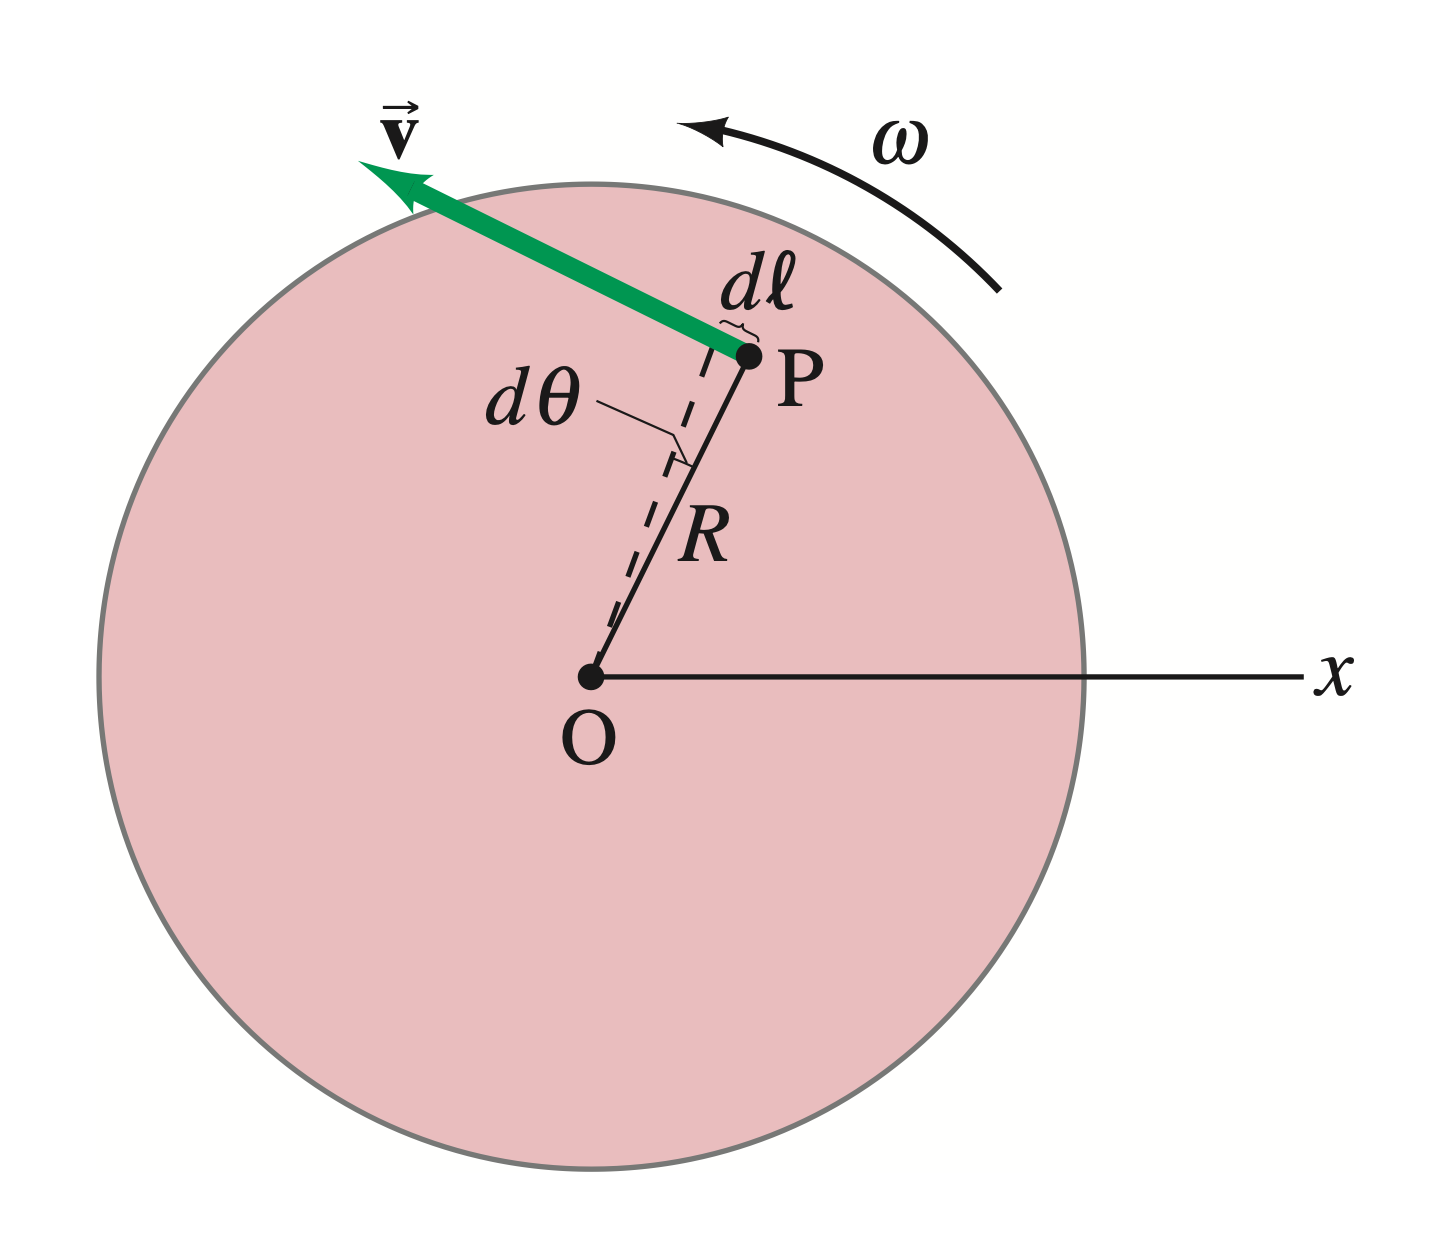
\includegraphics[scale = 0.225]{Images/Dynamica/RotatieCirkel.png}
%     \end{minipage}
% \end{theo}    

\begin{app}[Constante rotationele vs translationele versnelling]{Constante rotationele vs translationele versnelling}
    \vspace{-0.2cm}
    \begin{center}
        \def\arraystretch{2}
        \begin{tabular}{c|c}
            Rotationele beweging met constante $ \alpha $ & Translationele beweging  met constante $ a $ \\ \hline
            $ \omega = \omega_0 + \alpha t $ & $ v = v_0 +at $\\
            $ \theta = \omega_0t + \tfrac{1}{2}\alpha t^2 $ & $ x = v_0t + \tfrac{1}{2}at^2 $ \\
            $ \omega^2 = \omega_0^2 + 2\alpha\theta $ & $ v^2 = v_0^2 + 2ax $\\
            $ \omega_{gem} = \dfrac{\omega + \omega_0}{2}$ & $ v_{gem} = \dfrac{v+v_0}{2} $
        \end{tabular}
    \end{center}
\end{app}
 
\begin{theo}[Krachtmoment]{Krachtmoment}
    Het draaieffect (de hoekversnelling) van een kracht wordt bepaald door de grootte van de kracht, de richting/zin van de kracht en de `\textbf{momentarm}': afstand tussen het aangrijpingspunt van de kracht en de rotatie-as. Het \textbf{krachtmoment} is het rotationele equivalent van het translationele kracht, in formulevorm:

    \begin{equation*}
        \Vec{\tau} = \Vec{r} \times \Vec{F}
    \end{equation*}

    \noindent De grootte van het krachtmoment wordt gegeven door de volgende formule:

    \begin{equation*}
       \tau = rF\sin(\theta) = r(ma)\sin(\theta) = (m(r sin(\theta))^2)\alpha = I\alpha
    \end{equation*}

    % \noindent Sinds enkel de transversale component, de krachten, rotatie veroorzaken kunnen we de 2de wet van Newton toepassen, we vinden:

    % \begin{equation*}
    %     \tau_{net} = \sum_i \tau_i = I\alpha
    % \end{equation*}
\end{theo}

\begin{app}[Arbeid en Vermogen bij rotatie]{Arbeid en Vermogen bij rotatie}
    \begin{minipage}{.66\textwidth}
            De arbeid verricht door een object dat roteert rond een vaste as kan geschreven kan geschreven worden tegenover rotationele grootheden:
            \begin{equation*}
                W = \int \Vec{F} \cdot d\Vec{\ell} = \int F_{\perp}rd\theta
            \end{equation*}
            waarbij $ d\Vec{\ell} $ een infinitesimale afstand is loodrecht op $ r $ met grootte $ dl = rd\theta $. We weten van hierboven natuurlijk dat $ \tau = F_{\perp}r $, dus de formule wordt:
            \begin{equation*}
                W = \int_{\theta_1}^{\theta_2}\tau d\theta
            \end{equation*}
            Het vermogen bij rotatie kunnen we nu ook afleiden:
            \begin{equation*}
                P = \dfrac{dW}{dt} = \tau \dfrac{d\theta}{dt} = \tau \omega
            \end{equation*}
        \end{minipage} 
        \begin{minipage}{.33\textwidth}
            \centering
            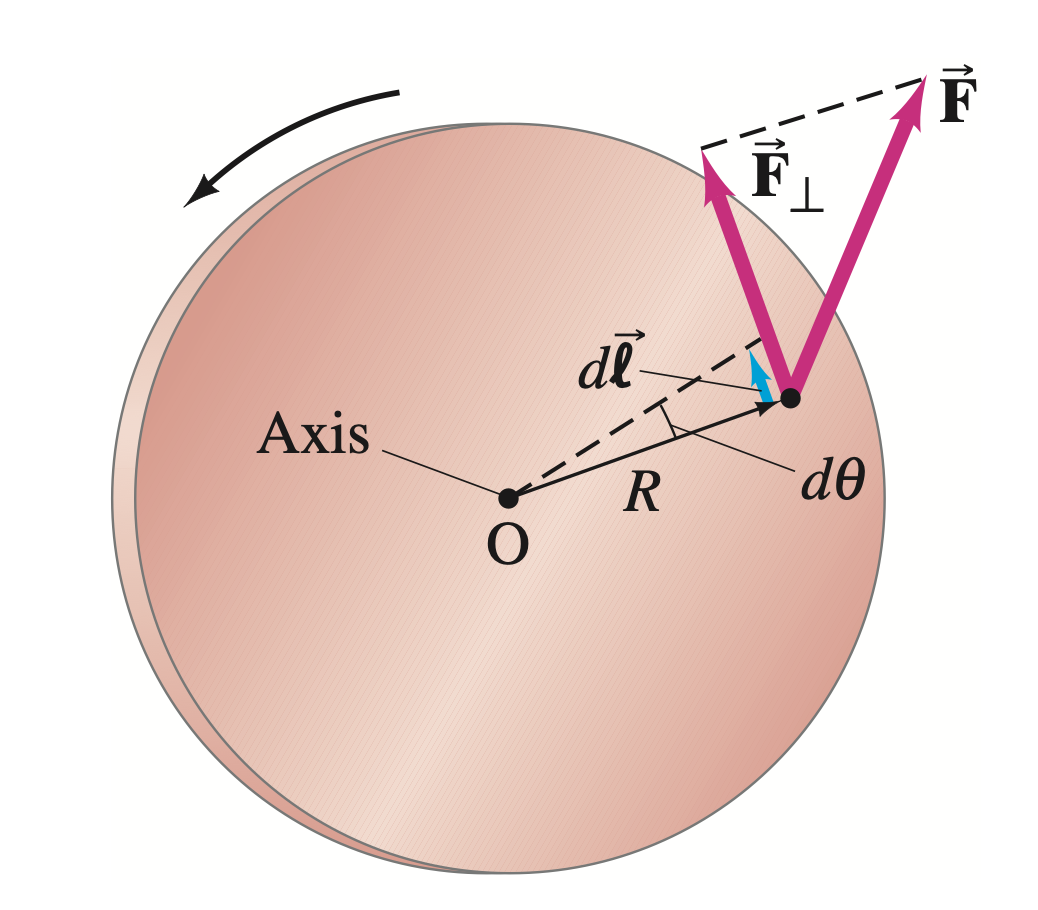
\includegraphics[scale = 0.25]{Images/Dynamica/ArbeidBijRotatie.png}
        \end{minipage}
\end{app}

\newpage

\begin{app}[Kinetische energie bij rotatie]{Kinetische energie bij rotatie}
    \vspace{-0.5cm}
    \begin{minipage}{.69\textwidth}
        Beschouw een stijf, roterend voorwerp als opgebouwd uit vele kleine deeltjes, elk met een massa $m_i$. De totale kinetische energie van het hele object is de som van de kinetische energie van alle deeltjes:
        \begin{equation*}
            K = \sum(\dfrac{1}{2}m_i v_i^2) = \sum(\dfrac{1}{2}m_i r_i^2\omega^2) =  \dfrac{1}{2}I\omega^2
        \end{equation*}
    \end{minipage} 
    \begin{minipage}{.27\textwidth}
        \centering
        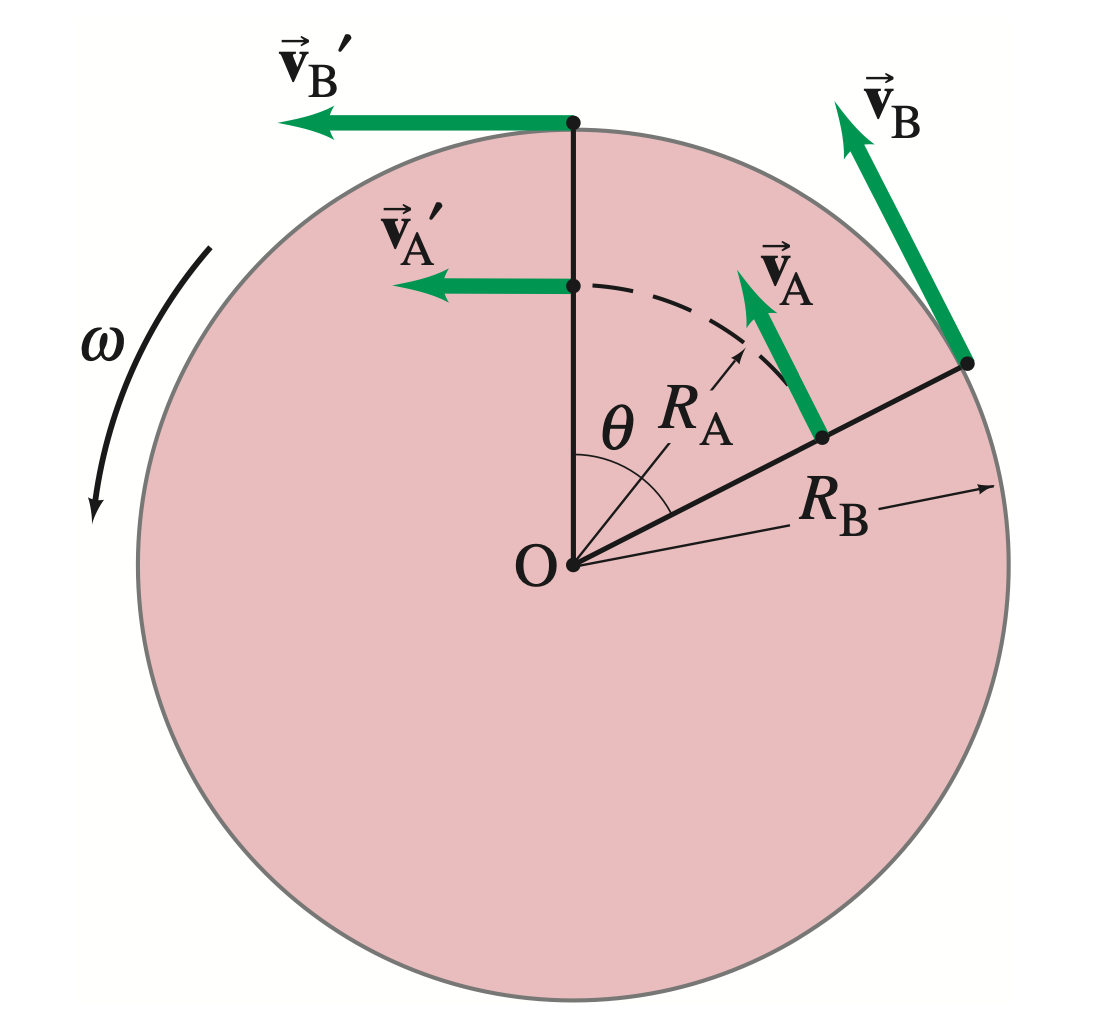
\includegraphics[scale = 0.15]{Images/Dynamica/SnelhedenOpRotatie.png}
    \end{minipage}
\end{app}

\begin{theo}[Impulsmoment]{Impulsmoment}
     Het \textbf{Impulsmoment} is de rotationele variant van het translationele impuls, net zoals krachtmoment rotationele variant is van de translationele kracht. Het wordt gegeven door de volgende formule:
    
     \begin{equation*}
         \Vec{L} = \Vec{r} \times \Vec{p}
     \end{equation*}

     \noindent De grootte van het impulsmoment kunnen we als volgt berekenen:
     \begin{equation*}
         L = p r \sin(\theta) = m v r \sin(\theta) = (m{(r \sin(\theta))}^2)\omega = I\omega
     \end{equation*}
     \vspace{-0.5cm}
\end{theo}

\begin{lem}[Behoud van impulsmoment]{Behoud van impulsmoment}
    De wet van de behoud van impulsmoment stelt dat de \textbf{totale impulsmoment} ($ \Vec{L}_{net} $) van een geïsoleerd stelsel van deeltjes constant is wanneer: 
    \begin{equation*}
         \tau_{net} = \sum \tau_{ext} = \sum \dfrac{I\omega}{dt} = \dfrac{dL_{net}}{dt} = 0
    \end{equation*} 
    \vspace{-0.5cm}
\end{lem}

\begin{vrg}[impuls – impulsmoment]{Vergelijking: impuls – impulsmoment}
    \begin{minipage}{.48\textwidth}
        \begin{center}
            
            \underline{Algemeen}: \\
            \vspace{0.25cm}
            \def\arraystretch{2.5}
            \begin{tabular}{c|c}
                impuls & impulsmoment \\ \hline
                $ \Vec{p} $ & $ \Vec{L} = \Vec{r} \times \Vec{p} $ \\ 
                $ \Vec{F} = \dfrac{d\Vec{p}}{dt} $ &  $ \Vec{\tau} = \dfrac{d\Vec{L}}{dt} $
            \end{tabular}
    
        \end{center}
    \end{minipage} 
    \begin{minipage}{.48\textwidth}
        \begin{center}
                
            \underline{Enkel bij een geïsoleerd systeem}: \\
            \vspace{0.25cm}
            \def\arraystretch{2.5}
            \begin{tabular}{c|c}
                impuls & impulsmoment \\ \hline
                behoud van impuls & behoud van impulsmoment \\ 
                $ F_{net} = \sum F_{ext} = 0 $ & $ \tau_{net} = \sum \tau_{ext} = 0 $
            \end{tabular}
        
        \end{center}
    \end{minipage}
\end{vrg}

% \begin{app}[Verband tussen impulsmoment en krachtmoment]{Verband tussen impulsmoment en krachtmoment}

%     Net zoals kracht zorgt voor de verandering van impuls van een voorwerp, zorgt krachtmoment voor de verandering van impulsmoment van een voorwerp: dit is het voornaamste verband.
    
%     Als we de tweede wet van newton bekijken bij rotatie, dan krijgen we de volgende formule die het verband aantoont:
    
%     \begin{equation*}
%         \sum \Vec{\tau} = I\Vec{\alpha} = I(\dfrac{d\Vec{\omega}}{dt}) = \dfrac{d(I\Vec{\omega})}{dt} = \dfrac{d\Vec{L}}{dt}
%     \end{equation*}

%     \noindent Omgekeerd kan ook als we een \textbf{puntmassa} bekijken:
%     \begin{equation*}
%         \dfrac{d\Vec{L}}{dt} = \dfrac{d(\Vec{r} \times \Vec{p})}{dt} = \dfrac{d\Vec{r}}{dt} \times \Vec{p} + \Vec{r} \times \dfrac{d\Vec{p}}{dt} = \Vec{v} \times \Vec{p} + \Vec{r} \times \Vec{F}
%     \end{equation*}
%     \noindent Het eerste lid van de som, namelijk $ \Vec{v} \times \Vec{p} $, wordt simpelweg 0, want $ \Vec{p} = m\Vec{v} $ is een lineaire combinatie van $ \Vec{v} $. Nu hebben we:
%     \begin{equation*}
%         \dfrac{d\Vec{L}}{dt} = \Vec{r} \times \Vec{F} = \tau \Rightarrow \dfrac{d\Vec{L}_{net}}{dt} = \Vec{r} \times \sum \Vec{F} = \sum \tau
%     \end{equation*}
%     % \noindent Als we nu $ \sum \Vec{F} $ pakken als de netto kracht, dan is bij een inertiaalreferentiestelsel:
%     % \begin{equation*}
%     %    \dfrac{d\Vec{L}}{dt} = \Vec{r} \times \sum \Vec{F} = \sum \Vec{\tau}
%     % \end{equation*}
%     \vspace{-0.5cm}
% \end{app}



